% This is based on "sig-alternate.tex" V1.9 April 2009
% This file should be compiled with V2.4 of "sig-alternate.cls" April 2009
%
\documentclass{report}

\usepackage[english]{babel}
\usepackage{graphicx}
\usepackage{tabularx}
\usepackage{subfigure}
\usepackage{enumitem}
\usepackage{url}


\usepackage{color}
\definecolor{orange}{rgb}{1,0.5,0}
\definecolor{lightgray}{rgb}{.9,.9,.9}
\definecolor{java_keyword}{rgb}{0.37, 0.08, 0.25}
\definecolor{java_string}{rgb}{0.06, 0.10, 0.98}
\definecolor{java_comment}{rgb}{0.12, 0.38, 0.18}
\definecolor{java_doc}{rgb}{0.25,0.35,0.75}

% code listings

\usepackage{listings}
\lstloadlanguages{Java}
\lstset{
	language=Java,
	basicstyle=\scriptsize\ttfamily,
	backgroundcolor=\color{lightgray},
	keywordstyle=\color{java_keyword}\bfseries,
	stringstyle=\color{java_string},
	commentstyle=\color{java_comment},
	morecomment=[s][\color{java_doc}]{/**}{*/},
	tabsize=2,
	showtabs=false,
	extendedchars=true,
	showstringspaces=false,
	showspaces=false,
	breaklines=true,
	numbers=left,
	numberstyle=\tiny,
	numbersep=6pt,
	xleftmargin=3pt,
	xrightmargin=3pt,
	framexleftmargin=3pt,
	framexrightmargin=3pt,
	captionpos=b
}

% Disable single lines at the start of a paragraph (Schusterjungen)

\clubpenalty = 10000

% Disable single lines at the end of a paragraph (Hurenkinder)

\widowpenalty = 10000
\displaywidowpenalty = 10000
 
% allows for colored, easy-to-find todos

\newcommand{\todo}[1]{\textsf{\textbf{\textcolor{orange}{[[#1]]}}}}

% consistent references: use these instead of \label and \ref

\newcommand{\lsec}[1]{\label{sec:#1}}
\newcommand{\lssec}[1]{\label{ssec:#1}}
\newcommand{\lfig}[1]{\label{fig:#1}}
\newcommand{\ltab}[1]{\label{tab:#1}}
\newcommand{\rsec}[1]{Section~\ref{sec:#1}}
\newcommand{\rssec}[1]{Section~\ref{ssec:#1}}
\newcommand{\rfig}[1]{Figure~\ref{fig:#1}}
\newcommand{\rtab}[1]{Table~\ref{tab:#1}}
\newcommand{\rlst}[1]{Listing~\ref{#1}}

% General information

\title{Project Title\\
\normalsize{Distributed Systems -- Project Proposal}}
\subtitle{subtitle}

% Use the \alignauthor commands to handle the names
% and affiliations for an 'aesthetic maximum' of six authors.

\numberofauthors{6} %  in this sample file, there are a *total*
% of EIGHT authors. SIX appear on the 'first-page' (for formatting
% reasons) and the remaining two appear in the \additionalauthors section.
%
\author{
% You can go ahead and credit any number of authors here,
% e.g. one 'row of three' or two rows (consisting of one row of three
% and a second row of one, two or three).
%
% The command \alignauthor (no curly braces needed) should
% precede each author name, affiliation/snail-mail address and
% e-mail address. Additionally, tag each line of
% affiliation/address with \affaddr, and tag the
% e-mail address with \email.
%
% 1st. author
\alignauthor \normalsize{Valentin Trifonov}\\
	\affaddr{\normalsize{ETH ID 13-941-679}}\\
	\email{\normalsize{vatrifon@student.ethz.ch}}
% 2nd. author
\alignauthor \normalsize{Simon Ringeisen}\\
	\affaddr{\normalsize{ETH ID XX-XXX-XXX}}\\
	\email{\normalsize{rsimon@student.ethz.ch}}
% 3rd. author
\alignauthor \normalsize{Jan Eberhardt}\\
	\affaddr{\normalsize{ETH ID XX-XXX-XXX}}\\
	\email{\normalsize{ebjan@student.ethz.ch}}
\and
% 4th. author
\alignauthor \normalsize{Caroline Creidenberg}\\
	\affaddr{\normalsize{ETH XX-XXX-XXX}}\\
	\email{\normalsize{ccreiden@student.ethz.ch}}
% 5th. author
\alignauthor \normalsize{Fabian Ulb}\\
	\affaddr{\normalsize{ETH ID XX-XXX-XXX}}\\
	\email{\normalsize{fabianu@student.ethz.ch}}
% 6th. author
\alignauthor \normalsize{Felix Wolf}\\
	\affaddr{\normalsize{ETH ID XX-XXX-XXX}}\\
	\email{\normalsize{fewolf@student.ethz.ch}}
}


\begin{document}

\maketitle

\begin{abstract}
In this document we are describing the initial planning of an app, which purpose it is to serve as a quick and easy way for people in an emergency situation to call for help to people within their vicinity. Our main goal is to provide a reliable service that informs people that are near an emergency as quick as possible.
\end{abstract}

\section{Introduction}

Traditional emergency solutions tend to have one issue making them unsuitable for many modern emergency situations, that is the need for a longer conversation about the problem with an officer and the long response latency. In some situations, much faster help is needed.
We try to tackle this problem by providing an application which is very easy and fast to start, issuing an alert to people nearby informing them of the emergency as well as the location, and therefore enabling people helping people where needed, even in situations where an internet connection might not be available.

As good as this sounds, there are a number of challenges to solve for this, particularly concerning fast and reliable multicasts and consistency for proximity-based communication.

First of all, there is the problem of reliability - in an emergency situation, you want to have your alert reaching other people by any means possible. We try to tackle this by using multiple different means of communication and detection:
First of all, with a working internet connection, we will pursue a centralized approach, a firebase database to store the locations of people and a server to evaluate the location informations and send push notifications via Google Cloud Messaging (GCM) to notify people in the vicinity of the alert origin. Firebase is a scalable real-time database which was originally developed by an independant company and later got bought by google~\cite{firebase}. We choose this approach for scalability reasons. See section 2.1 for more details. This provides a large range as well as a reliable way of communication.

Secondly, without a working internet connection, we take a P2P approach. There is p2pkit~\cite{p2pkit}, a framework developed by a spinoff of the ETH, Ueppa, which is developed exactly for proximity-detection, and works even without an internet connection. Though this is a nice approach, the current development status of this framework might not be sufficient for our requirements. We started a first series of tests with modest results but we will evaluate our options here further. One consideration is to replace p2pkit with the Android Wifi-P2P framework~\cite{android_wifi_p2p} or use it as a supplement. In case we arrive at the decision that it is insufficient we will focus ourselves on the centralized approach and take P2P as a best effort offline approach. Consult Section 2.2. for more details.

The combination of these approaches should hence provide reliability on the edge what’s possible with currently available technology.

\section{System Overview}

This is the core of the proposal.
It is where you spell out your technical plan and explain the project design.
Expected evaluation/demonstration issues would also be addressed in this section.
Use helpful figures such as~\rfig{example} and~\rfig{system-overview},
explain the figures in the text where you reference them. 


\begin{figure}[h]
	\centering
    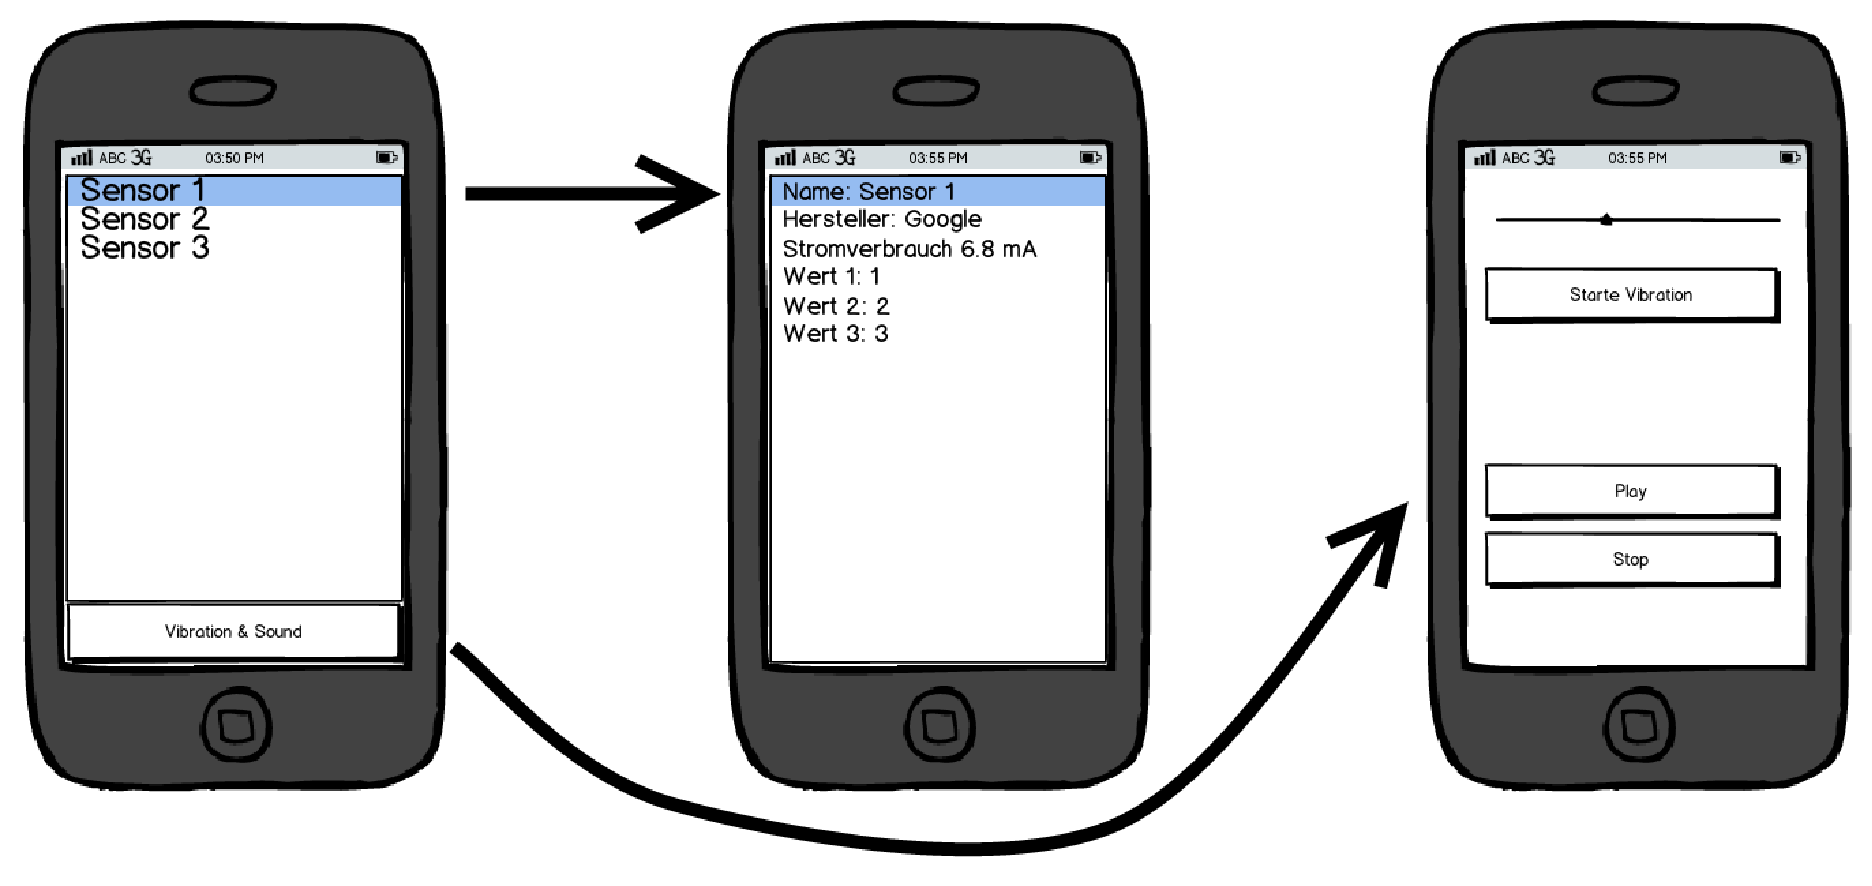
\includegraphics[width=\columnwidth]{example}
    \lfig{example}
    \vspace{-5mm} % use negative white space to fix too large gaps
	\caption{Only include useful figures. Do not simply copy something from a Web.}
\end{figure}



\section{Requirements}
Describe system setup, components, external libraries, hardware etc.


\begin{figure}[h]
	\centering
    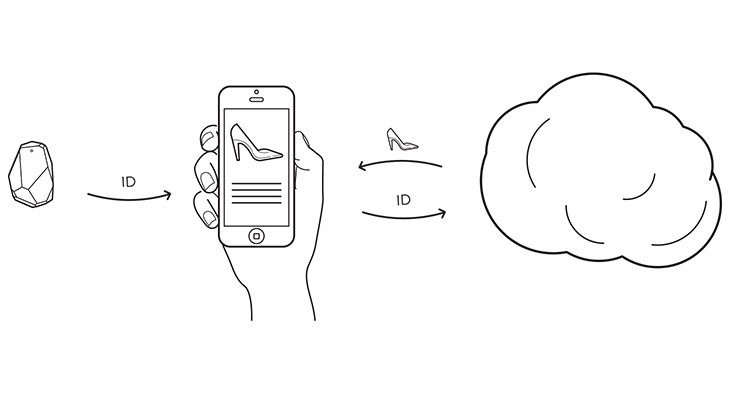
\includegraphics[width=\columnwidth]{overview.jpg}
    \lfig{system-overview}
    \vspace{-5mm} % use negative white space to fix too large gaps
	\caption{System Overview~\cite{estimote}}
\end{figure}

\section{Work Packages}
Breakdown the work to subtasks to meet the project requirements.
Define and describe these tasks.

\newcommand{\wpitem}[2]{\item\textbf{#1}\\#2}
\newcommand{\wpgroup}[2]{
    \item\textbf{#1}
    \begin{enumerate}[label*=\arabic*.]
        #2
    \end{enumerate}
}
\begin{enumerate}[label*=\arabic*.]
    \wpgroup{GUI \& Activities}{
        \wpitem{implement basic GUI}{}
        \wpitem{Structure the project}{provide interfaces for the different work packages}
        \wpitem{(Optional) Alarm Feedback \& Helper Proximity}{Add a feature where the one needing help receives feedback about people on their way to him and their distance}
    }
    \wpgroup{P2P backend}{
        \wpitem{P2P Test Phase, Basic Functionality}{
            test if the p2pkit is applicable for our needs (in terms of speed and reliability).
            If it is not, we will not pursue this option further
        }
        \wpitem{Discovery Logic}{implement discovering nearby people, keep track of peers in your vicinity}
        \wpitem{Alarm \& Revocation Logic (Snowball effect, Broadcast)}{implement sending and revoking alarms to nearby people and reacting to these events}
    }
    \wpgroup{Centralized Backend - Client Side}{
        \wpitem{Database Setup (Firebase)}{integrate a firebase db into our app, periodically update user location in the database}
        \wpitem{GCM integration}{}
        \wpitem{Server Interface}{Communication to the server and reacting to push notifications (send current location, start alarm)}
        \wpitem{Alarm logic}{check if alarm is still valid and user is in a useful range, react to alarm if nobody else already did, handle reaction of user}
        \wpitem{(Optional) Alarm Feedback \& Helper Proximity}{Add a feature where the one needing help receives feedback about people on their way to him and their distance}
    }
    \wpgroup{Centralized Backend - Server Side}{
        \wpitem{Implement server and integrate firebase db}{}
        \wpitem{GCM integration}{}
        \wpitem{Alarm Logic}{react to user alarm events and find nearby people}
        \wpitem{(Optional) Alarm Feedback \& Helper Proximity}{Add a feature where the one needing help receives feedback about people on their way to him and their distance}
    }
    \wpgroup{Miscellaneous}{
        \wpitem{Alarm Activation Logic}{implement a listener which monitors button events for a special combination and then triggers the alarm}
        \wpitem{always-on Android background process \& IPC}{figure out how to have the background code running in a separate process and how to communicate to it from the activities}
        \wpitem{(Optional) consider ways on how we could reduce spam alerts}{}
    }

\end{enumerate}
 
\section{Milestones}
The milestones section provides a work plan for carrying out the project.
This is your schedule for getting the project done.
Clearly state how the work packages will be distributed among the team members. 
% The following two commands are all you need in the
% initial runs of your .tex file to
% produce the bibliography for the citations in your paper.
\bibliographystyle{abbrv}
\bibliography{report}  % sigproc.bib is the name of the Bibliography in this case
% You must have a proper ".bib" file

%\balancecolumns % GM June 2007

\end{document}
